\Chapter{Képek közelítése a bemeneti vektorok terében}

A GAN által betanult térről nem kapunk egzakt információkat, nincs tudomásunk arról, hogy a modell hogyan helyezte el a sokdimenziós térben a tanult ismereteit. Egy betanított modell esetén csupán annyit látunk, hogy különböző random bemeneti vektorokra különböző képeket kapunk a generátor kimenetén.
Két random zajvektor között ha interpolálunk, akkor minden egyes mintavételezett pontból ki tudunk generálni olyan képeket, amelyek a két kép közti átmenetet jelentik és amelyeken megfigyelhetőek a két kép együttes tulajdonságai. A \ref{fig:interpolation} ábrán látható egy példa az interpolációra.

\begin{figure}[h]
\centering
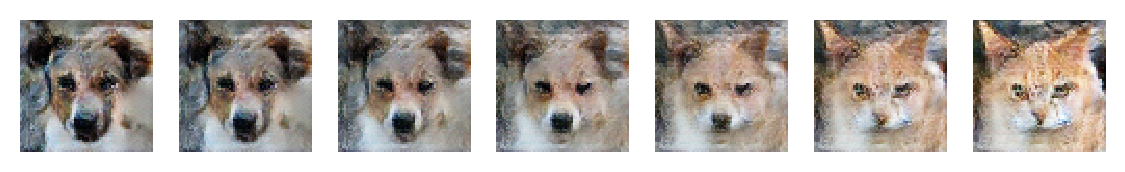
\includegraphics[width=15cm]{images/interpolation.png}
\caption{Generált képek lineáris interpolációval két zajvektor között}
\label{fig:interpolation}
\end{figure}

A bemeneti vektorok tere tehát folytonosan van kitöltve, bármely pontra egy képet kaphatunk vissza. Viszont ezen tér feltérképezése sem egy triviális feladat és az sem biztosított, hogy a tér az egymáshoz hasonló jellegzetességekkel van kitöltve.

A képek közelítésre egy megoldás lehet a \textit{synthesis-through-optimization}\cite{frans2021clipdraw} technika, amelyhez nem kell betanítani egy újabb modellt, csupán optimalizációs alapon történik meg a képek közelítése.
A technikához szükségünk van egy célfüggvényre, amelyre az optimalizációt végre tudjuk hajtani egy megjelenítőre, amely esetünkben a GAN generátora lesz és egy olyan eszközre, amellyel mérni tudjuk a kigenerált képek jóságát. Az utóbbi eszköz általában egy osztályozó szokott lenni, amelynek a tudásával bejárhatjuk a vizsgált teret. Az optimalizálást pedig a gradiens keresés módszerével szokás végrehajtani.
A CLIP \cite{radford2021learning} zero-shot osztályozó igen közkedvelt az ilyen fajta vizsgálatok elvégzésére. Az osztályozó kimenetén szabad szöveges mondatok jelennek meg a vizsgált képekre a megfelelő valószínűségi értékekkel kiegészítve. A CLIPDraw-ban \cite{frans2021clipdraw}  például nem is GAN modellt használtak a képek generálására, hanem csupán Bézier-görbék halmazán végezték el az optimalizálást és eredményül rajzokhoz hasonló képeket kaptak. Esetükben a célfüggvény a bemeneti mondatok és a CLIP osztályozó által kiadott mondat koszinuszi távolságának minimalizálása volt. A keresés végén a görbék olyan alakban rendeződtek, amelyek legjobban reprezentálják a bemeneti szabad-szöveges mondatot a CLIP osztályozó szerint.

A GAN $G$ generátorának bemenete egy $\vec{z} \in \mathbb{R}^{z_n}$ vektor, ahol $z_n$ általában 100 szokott lenni. Vagyis a bemeneti vektor egy $z_n$ dimenziójú tér egy pontja. A 100 dimenzióban történő keresés igen nehéz lehet a hagyományos heurisztikus módszerekkel, mint például a hegymászó módszerrel. A hegymászó optimalizáló módszer során a célfüggvényt minimalizáljuk (vagy maximalizáljuk) a pont körüli tartomány mintavételezésével, majd a megfelelő szomszédos pontra való lépéssel. A bemeneti paraméter lehet a pont kiinduló pozíciója, a lépésköz és a mintavételezés sűrűsége. A megfelelő pontosság érdekében igen sok mintára lehet szükségünk és ez egy sokdimenziós térben igen nagy lehet. A módszer hátránya lehet a fix lépésköz is, amely hatására lokális optimumokban ragadhatunk, ha a vizsgált felületünk bonyolult. Több vizsgálandó pont elszórása a térben megnövelheti az esélyét annak, hogy rátalálunk a globális optimumra is, viszont ez jelentősen megnöveli a számításigényt.
A gradiens módszer vagy gradient süllyesztés (\textit{Gradient Descent}) egy olyan iteratív optimalizáló módszer, amely a diferenciálható függvény lokális minimumának megtalására irányul. A célfüggvény elsőrendű deriváltjai igazítják el a vizsgált pontunkat a minimumhoz.

Egy kiválasztott kép közelítése a bemeneti vektorok terében az alábbi módon történhet:\\ 
Jelölje $X$ a keresendő képet, $G$ a generátort, $\vec{z} \in \mathbb{R}^{z_n}$ pedig a látens vektort.\\
A cél egy olyan $\vec{z} \in \mathbb{R}^{z_n}$ látens vektor keresése, amellyel az alábbi távolság minimalizálható.

$$ \min\left(\sum_{i=1}^{n\times m}\sqrt{(X_i-G(\vec{z})_i)^2}\right)$$

A képeket tehát pixelszinten hasonlítjuk össze kiindulásképp. Ez a távolságot szokás L2 távolságnak is nevezni, az L2 norma alapján, vagy euklideszi távolságnak is.
Egyéb metrikákat is alkalmazhatunk a képek hasonlóságának mérésére, ilyen a PCA, a HOG, MSE, stb...

Legyen $l$ a lépésméret, $X \in \mathbb{R}^{n\times m \times 3}$ a keresendő kép, $G$ pedig a betanított generátor.
\begin{enumerate}
	\item Generáljunk egy képet az aktuális $\vec{z}$ zajvektorral
$$\hat X = G(\vec{z})$$
	\item Számoljuk ki a generált kép és a keresendő kép távolságát.
$$ loss = \sum_{i=1}^{n\times m}\sqrt{(X_i-\hat X_i)^2} $$
	\item Számoljuk ki a gradienseket a hibafüggvény szerint
$$ \vec{grad} = \frac{d}{d\vec{z}} \left[loss\right]$$
	\item Módosítsuk a $\vec{z}$ zajvektor elemeit a kapott gradiensek szerint egy $l$ hosszúságú lépéssel
$$ z_i = z_i - (l \cdot grad_i)$$
	\item Ismételjük meg az algoritmust a konvergálásig.
\end{enumerate}

Azt, hogy pontosan mikor kell befejeznünk az algoritmust nincsen meghatározva előre. A hibafüggvények változát esetleg nyomon követhetnénk, és ha két érték között oszcillál a hibafüggvény, akkor valószínűleg elért az algoritmus egy lokális minimumot. A példa egyszerűsítése kedvéért a lépésszám is egy bemeneti paraméter jelen esetben.

Az algoritmus Tensorflow-ban történő megvalósítása a következő:

\begin{python}
random_noise = tf.random.uniform([1, latent_dim], minval=-1, maxval=1)
noise = tf.Variable(random_noise)
step_size = 0.03
steps = 50
for i in range(steps):
    with tf.GradientTape() as g_tape:
        g_tape.watch(noise)
        generated_image = generator(noise, training=False)
        loss = tf.norm(goal_image - generated_image)
    gradients = g_tape.gradient(loss, noise)
    noise = noise - (step_size * gradients)
\end{python}


Momentummal való kiegészítés:

Jelöljük $t$-vel az időpillanatot.

$$ z_i^t = z_i^{t-1} - (l \cdot f'(z_i^{t-1})$$

$$ valtozas^t = l \cdot f'(z_i^{t-1}) $$

$$ z_i^t = z_i^{t-1} - valtozas^t $$


Momentum esetén a változás:
$$ valtozas^t = l \cdot f'(z_i^{t-1}) + momentum \cdot valtozas^{t-1}$$


momentum 0 - 1 között (0 esetén sima gradient descent)


\begin{figure}[h]
\centering
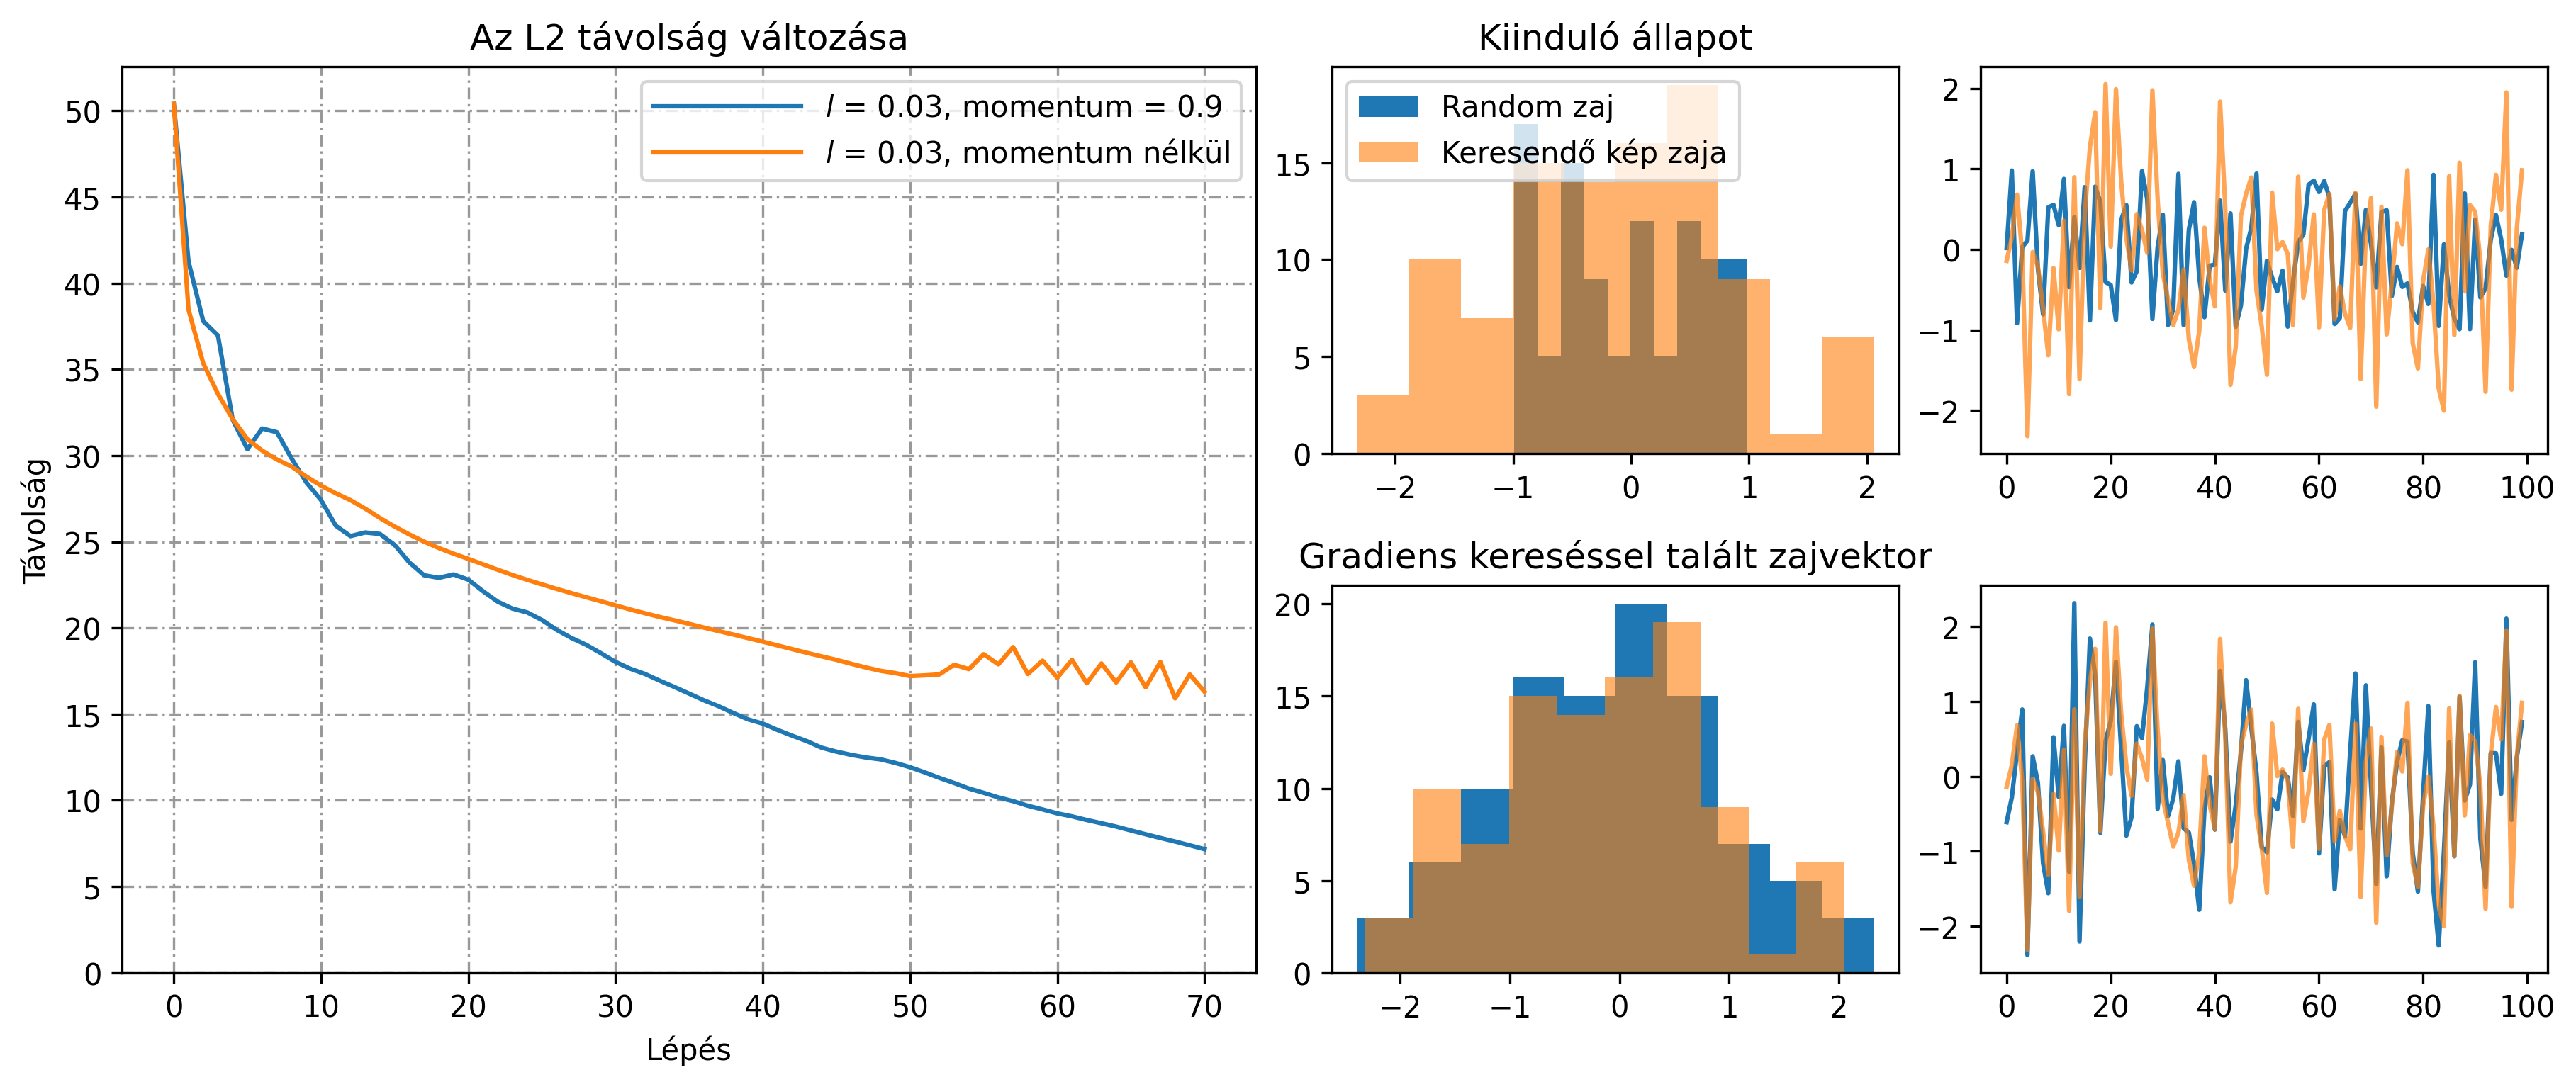
\includegraphics[width=15cm]{images/grad_losses.png}
\caption{A hibafüggvény változása a lépések során}
\label{fig:gradlosses}
\end{figure}


\begin{figure}[h]
\centering
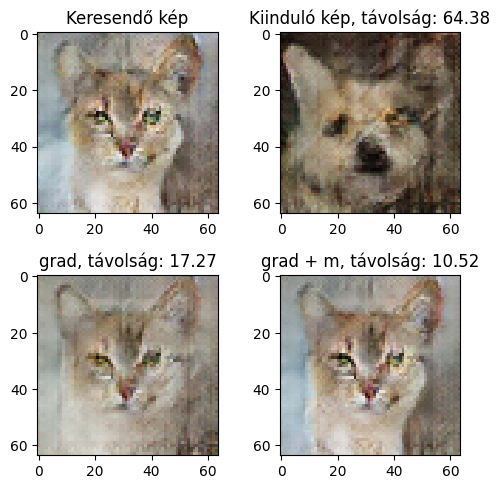
\includegraphics[width=8cm]{images/grad_found.png}
\caption{Gradiens kereséssel visszakeresett képek}
\label{fig:gradfound}
\end{figure}
